\documentclass[journal]{IEEEtran}
\usepackage{amsmath,amssymb,amsfonts}
\usepackage{tabularx}
\usepackage[utf8]{inputenc} % allow utf-8 input
\usepackage[T1]{fontenc}    % use 8-bit T1 fonts
\usepackage{url}            % simple URL typesetting
\usepackage{booktabs}       % professional-quality tables
\usepackage{amsfonts}       % blackboard math symbols
\usepackage{nicefrac}       % compact symbols for 1/2, etc.
\usepackage{microtype}      % microtypography
\usepackage{graphicx}
\usepackage{float}
\restylefloat{table}
\usepackage{hyperref}
\usepackage{multicol}
\usepackage{caption}
\usepackage{subcaption}
\usepackage{amsmath}
\usepackage{algorithm}
\usepackage{algpseudocode}
\usepackage{tikz}
\usetikzlibrary{trees}
\usepackage{listings}

\DeclareMathOperator*{\argmax}{arg\,max}  % in your preamble
\DeclareMathOperator*{\argmin}{arg\,min}  % in your preamble

\usepackage{textcomp}


%\usepackage[retainorgcmds]{IEEEtrantools}
%\usepackage{bibentry}
\usepackage{xcolor,soul,framed} %,caption

\usepackage[noadjust]{cite}
%\usepackage{biblatex}
%\bibliographystyle{plain}

\usepackage[font=small]{caption}

%=== TITLE & AUTHORS ====================================================================
\begin{document}
\bstctlcite{IEEEexample:BSTcontrol}
    \title{test}
\title{Accelerate Reinforcement Learning with Protective Boundaries}

\author{ Zongqiang Pang,Liping Bai ~\IEEEmembership{Member,~IEEE,} \thanks{Nanjing Unversity of Posts and Telecommunications, College of Automation \& College of Artificial Intelligence, Nanjing, Jiangsu,210000 China email:zqpang@njupt.edu.cn}}
% ====================================================================
\maketitle
% === ABSTRACT ====================================================================
% =================================================================================
\begin{abstract}
Protective Boundary is a common concept for atheletic training. Gymnast, divers, figure skaters would wear harness or a coach would be present to prevent falling and injuries. The same is true for children, as parents caringly provide a helping hand instead of just letting kids try things out themselves. Reinforcement Learning is an extention of approximate dynamic programming to circumstances where the system dynamics is unknown. With the newly added function approximation capacity brought about by deep learning, deep reinforcement learning is proven to be a formitable force when it comes to control. However, there is a clear difference between reinforcement learning and human learning. While out joints can have all kinds of combinatorial movement, we only use a few of those even in the most rigirous scenarios such as yoga. It seems to us that there are tools such as protective boundaries that human use to accelerate our learning. Is there a way to minimize the inefficiencies present in reinforcement learning and get closer to human level efficiency? Immitation learning seek to address this issue by provide a model trajectory, and meta-learning see to address this by provide agents with a sense of physics. In this paper, we mimic the Protective boundary method we see in atheletic training to provide agents additional clues about the environment. There are two advantages in this proposed scheme. First, the Protective boundary prevent premature termination of an episode, which is of particular importance to environment where failure is costly. Second, the Protective boundary method accelerate data collection on states/action pair that matters. We implemented the proposed prohibitibe boundary scheme on various OpenAI Gym environments, and for all the experiments carried out, Protective boundary has shown to accelerate training. All the code and data can be found at: \href{https://github.com/BaiLiping/ProtectiveBoundary}{Code Deposite}
\end{abstract}
% === KEYWORDS ====================================================================
% =================================================================================
\begin{IEEEkeywords}
Reinforcement Learning, Assisted Reinforcement Leraning, Reward Engineering, Safe Exploration
\end{IEEEkeywords}
\IEEEpeerreviewmaketitle
% === I. Paper =============================================================
% =================================================================================
\section{Introduction}
\IEEEPARstart{R}{einforcement} learning(RL) is the process of methotically extracting information from experiments to gradually bound policy distributions, maximizing the expected reward along a path. RL can be seen as approximate dynamic programming extended to unknow system dynamics, powered with statistical methods and neural networks.When the first batch of reasonable RL results were introduced, they were met with coldness by people in control community. The preface of Bertseka's book Neuro Dynamic Programming provides a good sample on how reinforcement learning is perceived by the control community back in 1996: "...These methods (Reinforcement Learning) were aiming to provide effective suboptimal solutions to complex problems of planning and sequential decision making under uncertainty, that for a long time were thought to be intractable. Our first impression was that the new methods were ambitious, overly optimistic, and lacked firm foundation....Three years later, after a lot of study, analysis, and experimentation, we believe that our initial impressions were largely correct." \cite{Bertsekas1996NeuroDynamicP}

Things are dramatically different today. RL community routinely generates results that seem untainable to traditional control methods. What has changed is not the theoretical foundation of RL, which is as leaky as it was in 1996, but its computational infrastructure. Before 2010, the predominent tools for function approximation are kernel methods, where feature spaces are used to transform nonlinear functions into linear space such that regression can be performed. Today, the default function approximator are neural networks. Another major change in computation is that of GPU based acceleration. Before the advent of CUDA, GPU programming requires PhD in computer graphics. Today, anyone who is proficient in C/C++ can programme GPU to parallelize their compuation. Software packages such as PyTorch and Tensorflow made this even easier.

However, there are clearly aspects of RL that is unreasonable yet papered over by fast computing. For instance, in order to train a humanoid to stand up, the agent need to explore all the combitions of joints movements. Reward signals would provide cues the agent as of which joints combitions are most likely to result in high scores. While children do explore plenty when they learn stand up and walk, I have never seen anyone who is malleable and flexible enough to explore all the combinatorial possibilities of joints positions, not even baby yoga master if there is one. Human must learn more efficiently than does RL agents. That is what we hope to propose in this paper: a method to accelerate reinforcement learning based on our observation of human learning process, specifically, the protective boundaries utilized during atheletic training. As is shown by our experiment results, our methods does accelerate reinforcement learning in all the experimental environments. Further research is required to analyze where to set the protective boundary and with what parameter.

In section I we introduce reinforcement learning to control resaerchers. In section II we introduce our promosed protective boundary scheme for acclerated RL agent training. In section III, we detail the results of all our experiments. While the experiments are conducted in OpenAI Gym simulated environment, we designed things in a way such that this method can be implemented in physical world as well. In the final section, we conclude on what we have learnt from our experiments and lay out directions for further research.

\section{Reinforcement Learning For Control Researchers}

\subsection{A Note on Notations}
The first barrier stands between control researchers and RL is the notation system. Control communities use the notation system introduced by Lev Pontryagin. State is denoted by $ \mathcal{X}$, conventionally a letter representing the unknown. Action is denoted by $\mathcal{U}$, the first letter of Russian for action. The dynamics and stocasticity is captured by physical model constraints $x_{t+1}=f(x_t,u_t,e_t)$ where e denotes the noise of a system. The objective is usually to minimize the cost funtion $\mathcal{J(.)}$. Reinforcement Learning communities use the notation system introduced by Richard Bellman who studied dynamic programming. State is denoted $\mathcal{S}$, Action is denoted $\mathcal{A}$. The dynamics and stochaticity is captured via transition matrix $\mathcal{P}$ of a Markov Decision Process.The objective of RL is the maximize the reward function $\mathcal{R(.)}$. We would like to present this note to control researchers at the begining of our paper as they might find the reinforcement learning literature notation rather confusing.

\subsection{From Approximate Dynamic Programming to RL}

Reinforcement Learning is not a new subject, control researchers probably know it by the name Approximate Dynamic Programming. Dynamic Programming is simply reasoning backwards. Take trajectory optimization for instance, if we know the desired final state and system constraints then we can simply compute backwards on the penultimate step, and the computing chain flows backwards from there. The prerequisites for a successful dynamic programming based controller are two-pronged: first, the observation space and action space are reasonably small; second, the system dynamics function is known. Neither is easily met in real life scenario.

Approximate Dynamic Programming comes in when the action space and observation space are large. Instead of computing for exact one to one relationship between observation and action choice, we use a function approximator to capture all the control information. Yet even for approximate dynamic programming, the reasoning backwards requires knowing system dynamics function. RL finally provides the bridge to extend approximate dynamic program to circumstances when the system model is unknow.

In order to introduce RL to control researchers, we framed RL in the language of optimization. Broadly speaking, there are three revenues where neural network based approximation finds its way into optimization as shown in figure \ref{fig:1}.

\begin{figure}
    \centering
    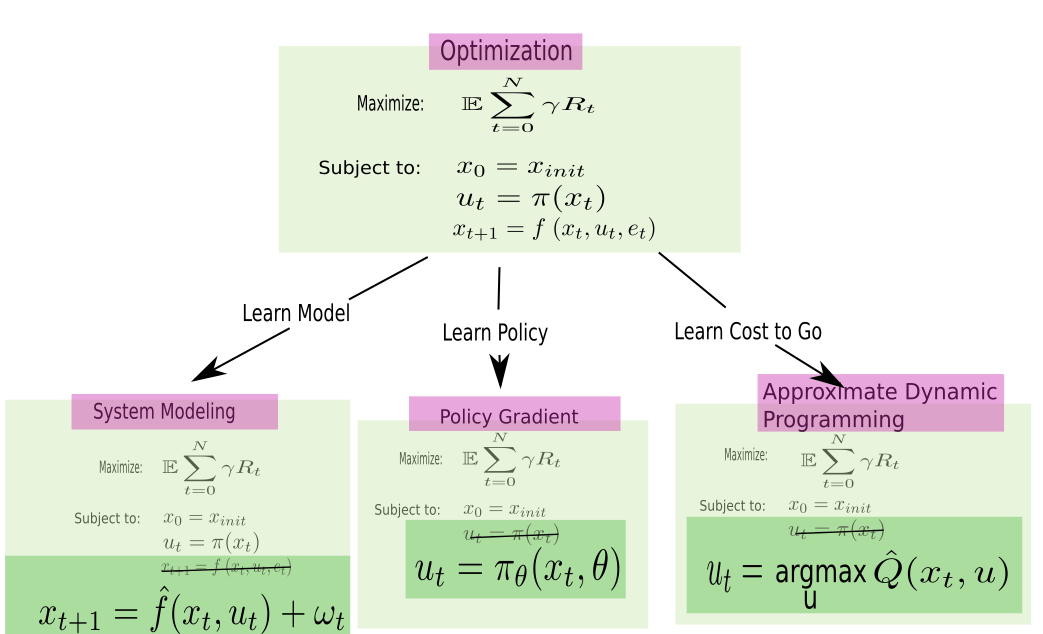
\includegraphics[width=0.5\textwidth]{Control.png}
    \caption{From Optimization to Learning}
    \label{fig:1}
\end{figure}
Neural Networks can be used to approximate system dynamics function, which is topic for System Identification researchers. While it is true that model based reinforcement learning and offline learning has gain tractions in recent years, in this paper, we won't focus on this line of research. Neural Netoworks can also be used to approximate control policy and the cost-to-go in approximate dynamic programming. A bootstrap structure is the most critical step in extending approximate dynamic programming to cases where the system function is unknow. Cost-to-go, which is computed based on system dynamics is used in order to choose an action. In RL, the agent just guess the cost-to-go and make choices according to its guesses. As the agent accumunate data based on our guesses, it refines the process it utilizes to come up with estimations. To put this process simply: when an agent learns to control an unknown system, it made assumptions on the steps ahead and base its action on those assumptions. After observing experiments data, the agent calibrate its ability to guess.

\subsection{Combine Policy Approximation and Cost-to-go Approximation}
\subsubsection{Advantage Actor Critic(A2C)}
\subsubsection{Trust Region Actor Critic}
\subsubsection{PPO}
\subsection{Entropy Regularization}
\section{Protective Boundary}
\subsection{Protective Boundaries in Atheletic Training}
Have you ever wondered how do world class athelets such as gymnists, figure skaters, divers accomplish feats that are seemingly impossible to us ordinary human?  While bruises, torn ligaments, broken bones, even concausion are part of being an athelete, those injuries are by no means trivial and should be minimized at all cost. Should athletes train the same way as would reinforcement learning agents, they will be dead or so severely injured long before they can pick up any skill. Protective Boundaries, implemented with either human coach or training harnesses is an integral part of atheletic skill acquisition process, as examplified by figure \ref{fig:athelete}. Detailed examples of how atheletes utilizes Protective boundary can be found \href{https://www.youtube.com/playlist?list=PLyqL4-20ZuTRo-DysDQBGDnwZsrySXP4b}{here}.

\begin{figure}
\centering
\begin{subfigure}{0.25\textwidth}
  \centering
  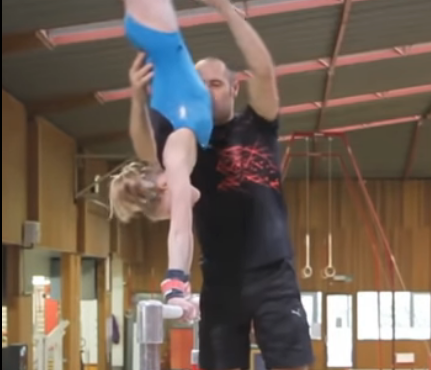
\includegraphics[width=\linewidth]{training1.png}
  \caption{Human Protective Boundary}
\end{subfigure}%
\begin{subfigure}{.25\textwidth}
  \centering
  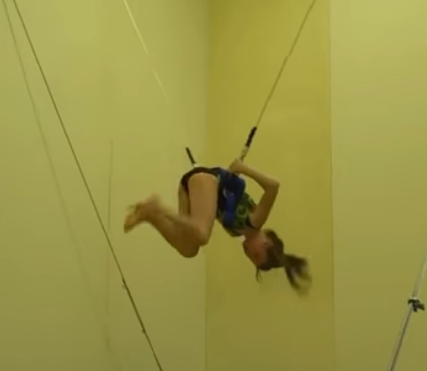
\includegraphics[width=\linewidth]{training2.png}
  \caption{Harness Protective Boundary}
\end{subfigure}
\caption{Protective Boundary in Atheletic Training}
\label{fig:athelete}
\end{figure}

\subsection{Implement Protective Boundary in OpenAI Gym}
We implemented our protective boundary experiments in OpenAI Gym as a proof of concept. We are cognicent of the fact that most of the control tasks facing our readers would be in real physical worlds. Therefore, we designed the protective barrier in a manner such that they can be swiftly adapted in real world should any researchers chooce to do so.

OpenAI Gym is a simulation environment build for reinforcement learning agents. Agent observe the state vector, reward, and termination after taking a step, which is implemented in the following sentense: observation, reward, done, info = environment.step(action).

There are various reinforcement learning agents implementations out there in the market. We choose tensorforce for this paper because it is routinely maintained, updated and with detailed instrictions on how each agent is constructed. We choose PPO agents for our experiments with entropy regularization. We set the parameters of the agents of the agents not to minimize the training steps but to accenturate the difference between our approach of training and that of normal training. Agents in the same environments share the same parameters, the only difference is weather or not they have protective boundaries.

Our experiments are conducted over the following environments: CartPole, with discrete action space; Inverted Pendulum, with continuous action space; Inverted Double Pendulum; Hopper; Walker. We did not implement our approach on more sophisiticated environments such as Humanroid and HumanroidStandup due to hardware constraints. Yet we feel that for the data we collected, our approach has shown acceleration on training when the boundaries are setup approapriately. Researchers with more powerful compute should check to see if our scheme works for environments that is harder to simulate.

One difficulty facing control researchers when they first interact with OpenAI Gym environment is the lack of documentations. We took the time to figure out what does agents observe in each environment and included the detailed notes in our code.

\subsection{CartPole and Inveretd Pendulum}
CartPole's Observation Space is: [Cart Position, Cart Velocity, Pole Angle, Pole Angular Velocity]. The discrete action space is for cartpole: [Push Cart to the left, Push cart to the right]. The continuous action space for Inverted Pendulum is an action ranging from -1 to 1, where -1 means the acturator moves the cart to the left with maximum power and 1 means the acturator moves the cart to the right with maximum power. The terminal states of cartpole is: when the absolute value of cart position is greater than 2.4 or when the absolute pole angle is greater than 12 degrees.

We proposed three protective rings anchored on the cart, at the height of middle of the pole, each allowing the pole to fall at maximum absolute value of 6,8.4,10.8 degrees respectively, as shown by the figure \ref{fig:cartpolePB}.

When the pole hit the protective boundary, it would push the cart back to the center, implemented by an automatic action choice of 0 or 1 depending on the sign of angle. A penulty is incurred every time the pole makes contact with the protective boundary, the penulties are set to be 0,-5,-7,-10,-12,-15 for each protective boundary. Our experiment result on cartpole are shown by figure \ref{fig:CartPole}. As the data suggest, when the boundary is set at 6 degree, it seems to be too restrictive for agent training. The best ressults is seen when the boundary is set at 10.8 degree, giving the agent plenty of rooms to adjust itself and acquiring the skill. The accelerated learning seems to be brought about mostly by the protective boundary itself instead of the penulty terms since our data suggest that when the boundary is set at the right place, all the penulties accelerate learning to a certain extend.

The experiment result for cartpole suggest simimar conclusion as shown by figure \ref{fig:InvertedPendulum}

\begin{figure}
     \centering
      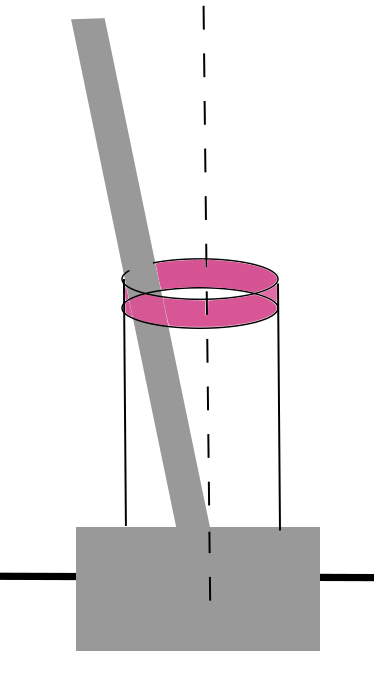
\includegraphics[width=0.1\textwidth]{cartpole1.png}
      \caption{CartPole Protective Boundary}
      \label{fig:cartpolePB}
\end{figure}

\begin{figure}
    \centering
    \captionsetup[subfigure]{font=scriptsize,labelfont=scriptsize}
    \begin{subfigure}[b]{0.5\textwidth}
      \centering
      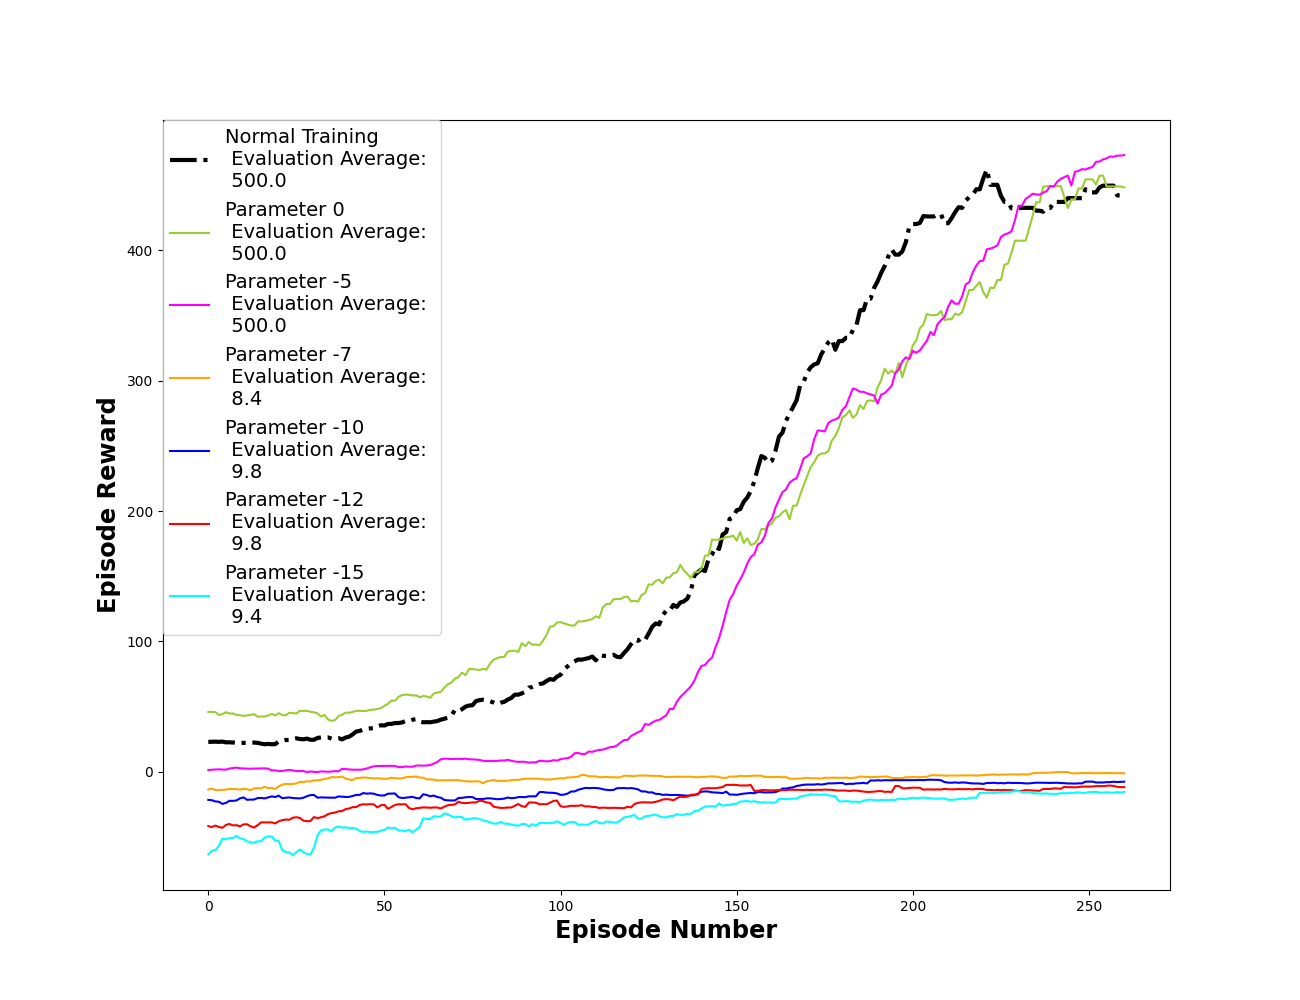
\includegraphics[width=\textwidth]{Cartpole_with_Boundary_at_0.5.png}
    \end{subfigure}
    \vspace*{0.0mm}
    \begin{subfigure}[b]{0.5\textwidth}
      \centering
      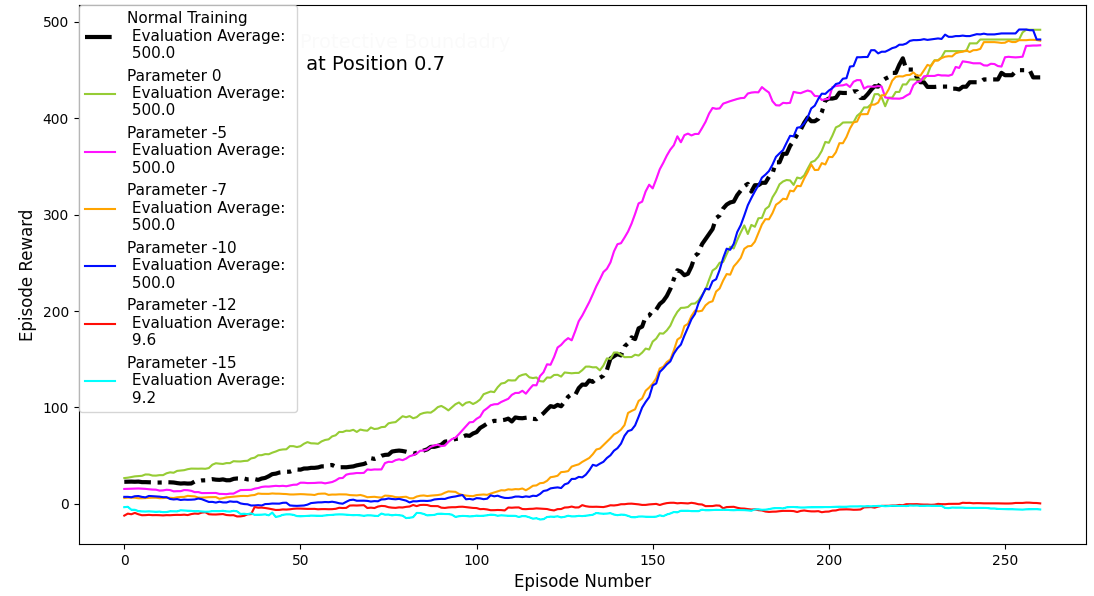
\includegraphics[width=\textwidth]{Cartpole_with_Boundary_at_0.7.png}
    \end{subfigure}
    \vspace*{0.0mm}
    \begin{subfigure}[b]{0.5\textwidth}
      \centering
      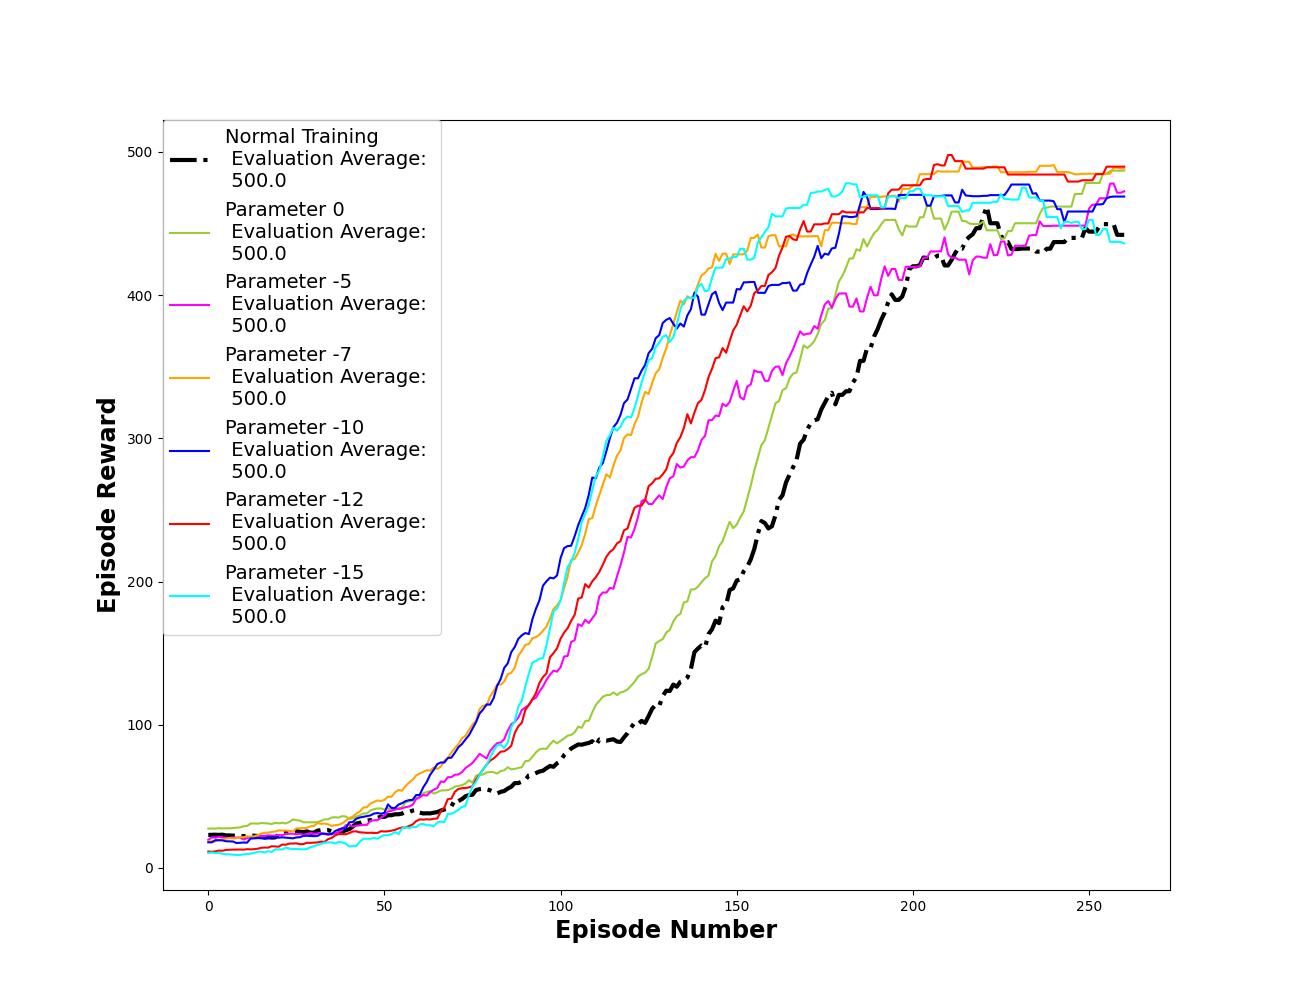
\includegraphics[width=\textwidth]{Cartpole_with_Boundary_at_0.9.png}
    \end{subfigure}
    \caption{CartPole Experiments}
    \label{fig:CartPole}
\end{figure}

\begin{figure}
    \centering
    \begin{subfigure}[b]{0.5\textwidth}
      \centering
      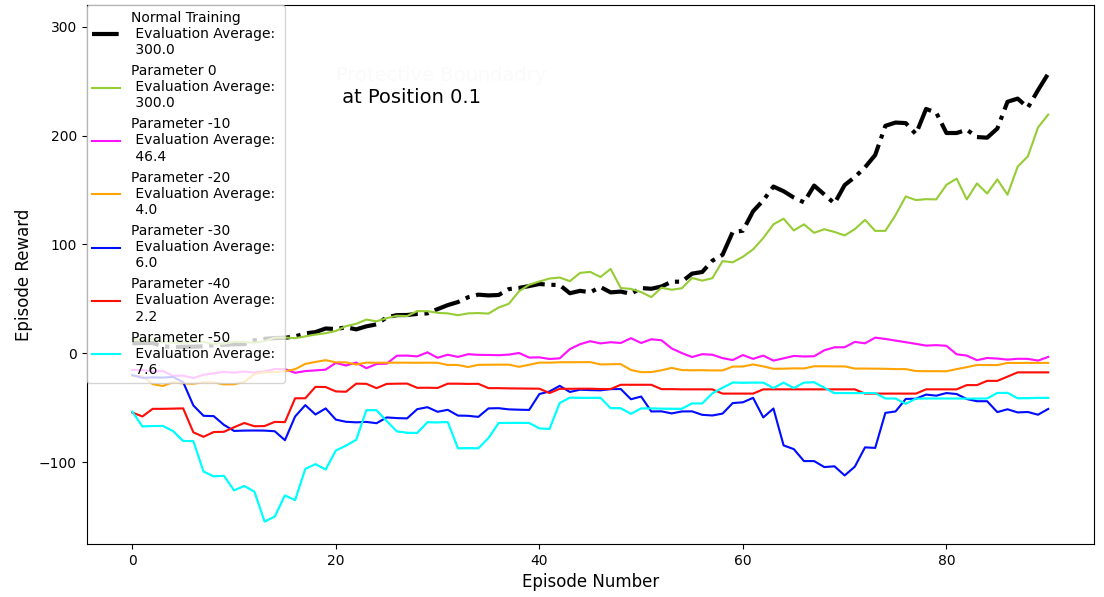
\includegraphics[width=\textwidth]{Inverted_Pendulum_with_Boundary_at_0.1.png}
    \end{subfigure}
    \vspace*{0.0mm}
    \begin{subfigure}[b]{0.5\textwidth}
      \centering
      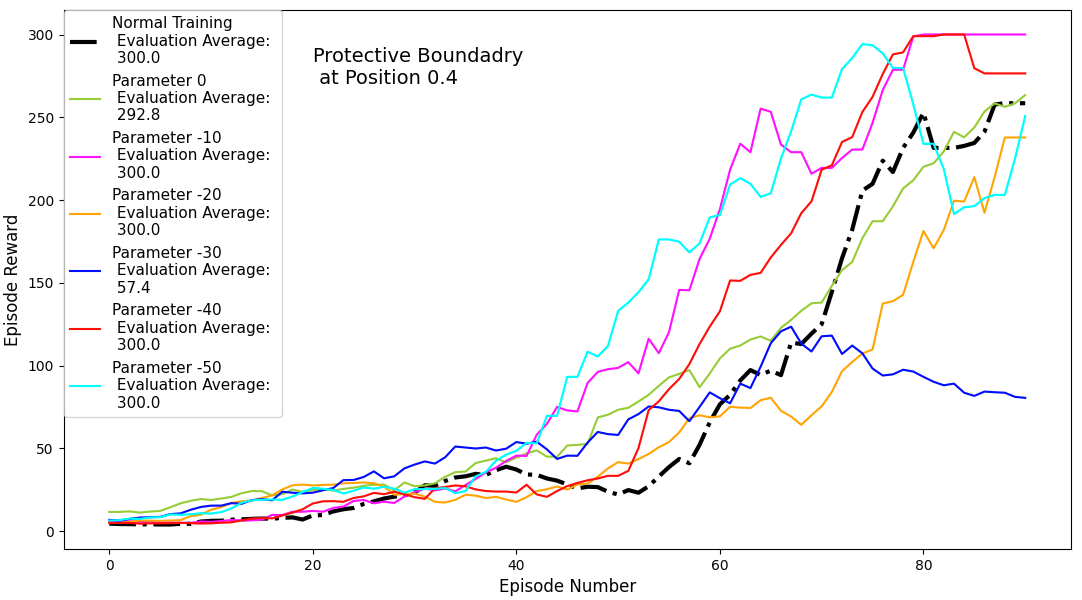
\includegraphics[width=\textwidth]{Inverted_Pendulum_with_Boundary_at_0.4.png}
    \end{subfigure}
    \vspace*{0.0mm}
    \begin{subfigure}[b]{0.5\textwidth}
      \centering
      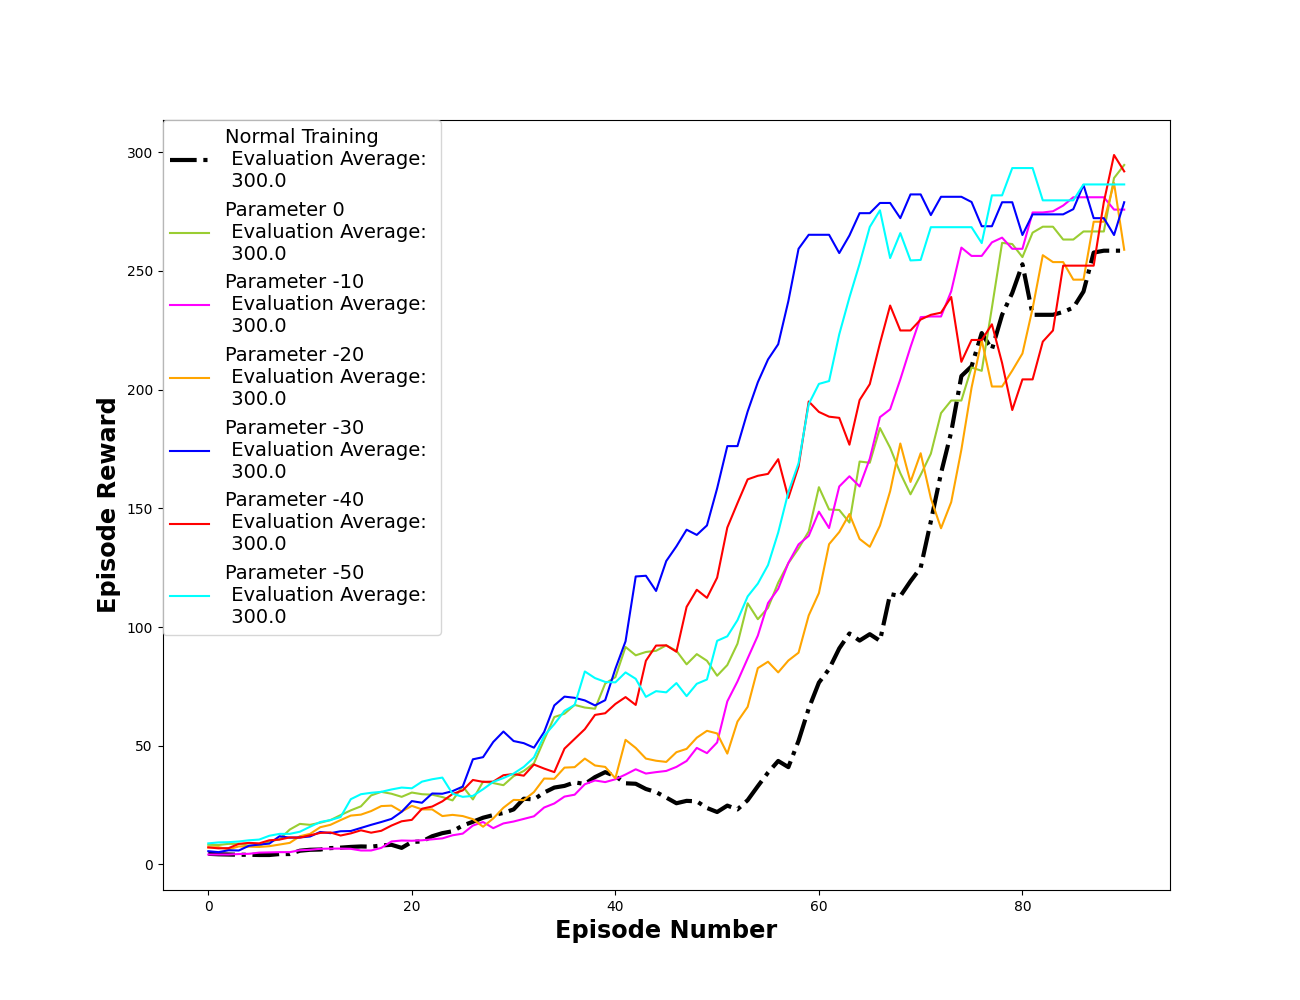
\includegraphics[width=\textwidth]{Inverted_Pendulum_with_Boundary_at_0.5.png}
    \end{subfigure}
    \caption{Inverted Pendulum Experiments}
    \label{fig:InvertedPendulum}
\end{figure}
\subsection{Inverted Double Pendulum}
The inveretd double pendulum has observation space as follows: [x position of the cart, sin($\theta_1$), sin($\theta_2$),cos($\theta_1$),cos($\theta_2$),velocity of x, angular velocity of $\theta_1$, angular velocity of $\theta_2$, constraint force on x, constraint force on $\theta_1$, constraint force on $\theta_2$]. $\theta_1$ and $\theta_2$ are the angles of the upper and lower pole perspectively.

The action space for Inverted Double Pendulum is an action ranging from -1 to 1, where -1 means the acturator moves the cart to the left with maximum power and 1 means the acturator moves the cart to the right with maximum power.

The Terminal state of double inveretd pendulum is when the y postion of the upper pole, which can not be observed by the agent falls below 1.

We design the protective boundary to be located at the same height as does the joint between upper and lower pole, as indicated by figure \ref{fig:doublePB}. The boundary allows the joint to flex for 0.4, 0.5 and 0.6 radians perepectively, each with the penulty parameters of a choice between 0,-3,-4,-5,-6,-7. When the joint extend to touch the protective boundary, an action of -1 or 1 would be automatically applied to rectify the situation, depending on the sigh of the angles.

\begin{figure}
     \centering
      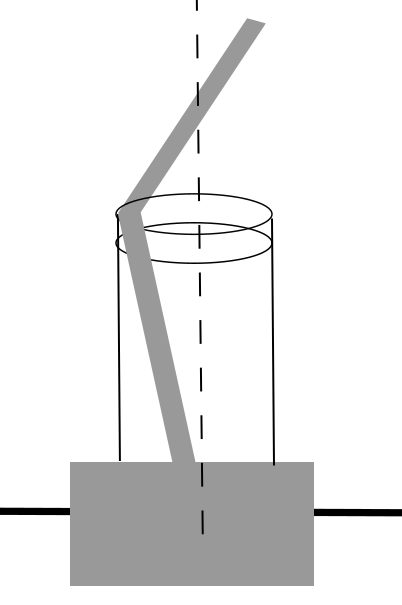
\includegraphics[width=0.1\textwidth]{cartpole2.png}
      \caption{Inveretd Double Pendulum Protective Boundary}
      \label{fig:doublePB}
\end{figure}

Our experiments result is show by figure \ref{fig:Double Pendulum} with conclusion similar to that of cartpole and inverted pendulum results. When the protective boundary is set at 0.4 radius, it hinders learning rather than facilitate it. When the boundary is set at 0.5 radius with a penulty parameter of -7, we see the most drastic acceleration of agent training. However, when the boundary is set at 0.6 radius, it seems to have given the agent too much flexibility since the result suggest that the acceleration is not as profound compare to that of boundary set at 0.5.

\begin{figure}
    \centering
    \begin{subfigure}[b]{0.5\textwidth}
      \centering
      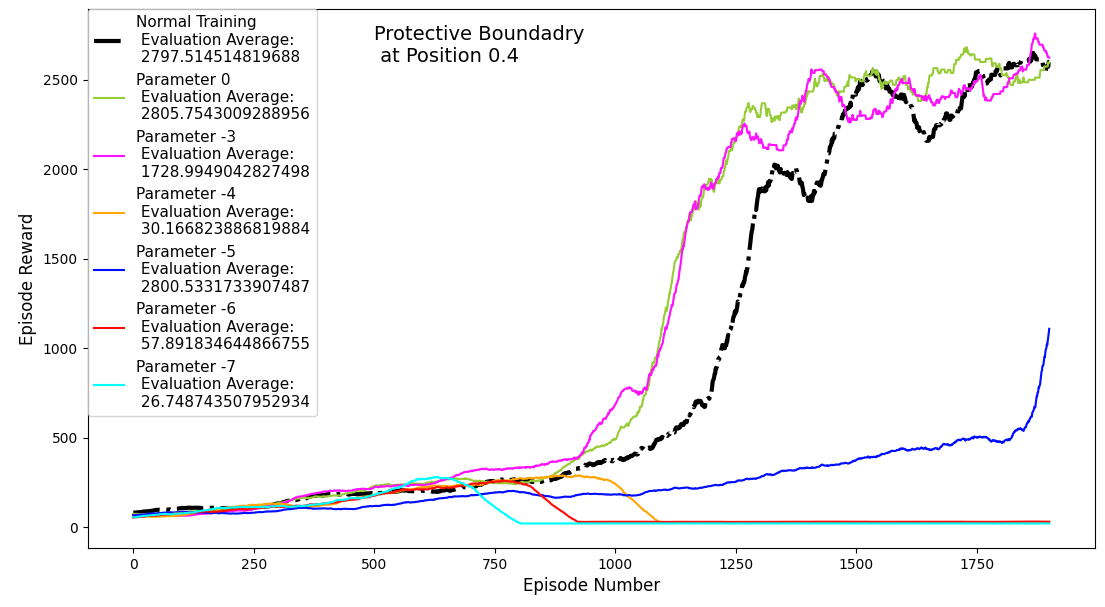
\includegraphics[width=\textwidth]{Double_Pendulum_with_Boundary_at_0.4.png}
    \end{subfigure}
    \vspace*{0.0mm}
    \begin{subfigure}[b]{0.5\textwidth}
      \centering
      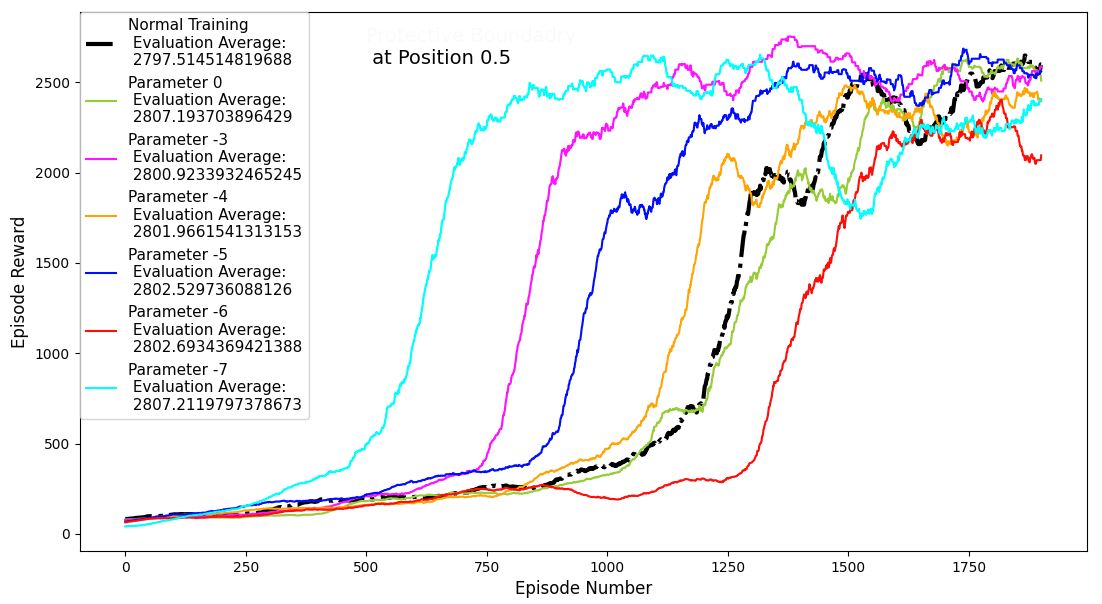
\includegraphics[width=\textwidth]{Double_Pendulum_with_Boundary_at_0.5.png}
    \end{subfigure}
    \vspace*{0.0mm}
    \begin{subfigure}[b]{0.5\textwidth}
      \centering
      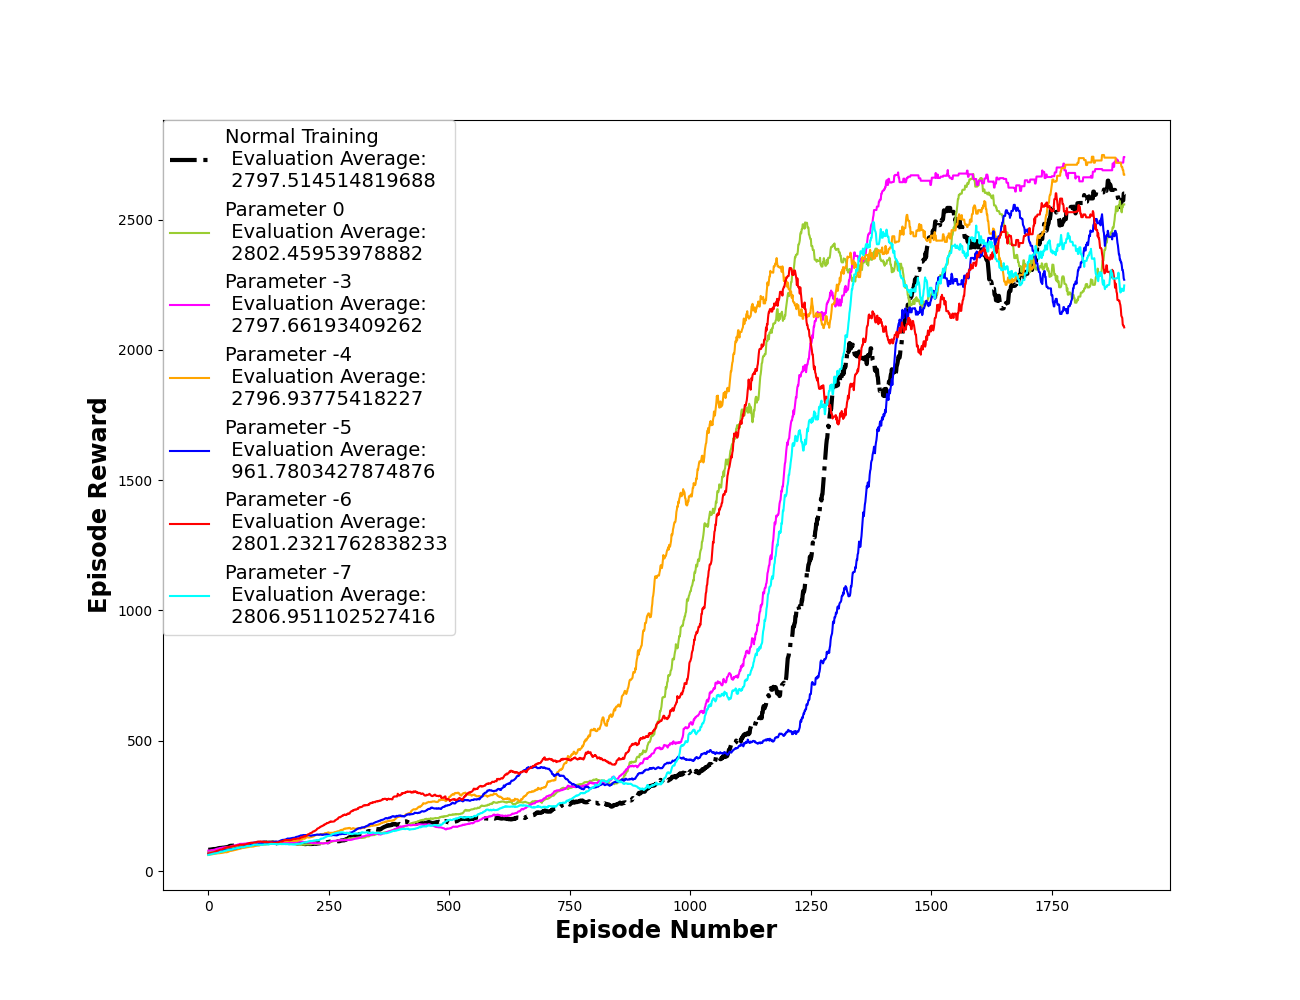
\includegraphics[width=\textwidth]{Double_Pendulum_with_Boundary_at_0.6.png}
    \end{subfigure}
    \caption{Inverted Double Pendulum Experiments}
    \label{fig:Double Pendulum}
\end{figure}


\subsubsection{Hopper}
The observation space of hopper is the following: [z position, y position, thigh joint angle, leg joint angle, foot joint angle, velocity at x axis, velocity at z axis, velocity at y axis, angular velocity of thigh joint, angular velocity of leg joint, angular velocity of foot joint].

The action space of hopper are three continuous action choices for three acturators [thigh acturator, leg acturator, foot acturator]. The range of for acturators are -1, which means apply force towards the negative direction with maximum power, and 1 which means apply force towards the positive direction with maximum power.

The terminal states for hopper are when the absolute y position is greater than 0.2.

The protective boundary is set with the y position at 0.05, 0.1 and 0.15, each with the penulty parameters that is chosen from 0,-3,-5,-7,-10. When the agent touches the protective boundary, we gentenly guide it slightly towards the smaller y position, and the velocities terms are all set to zero in this step. We seek to mimic how a coach would guide an atheletes towards the desired trajectory during training. When the athelete is about to fall, the coach would take over and apply the apppriate force such that the trajectory of that athelete is reset slightly and he or she get to experience more with states that are pertinent to his/her training.

Our experiment result is show by fiture \ref{fig:Hopper}. Similar to the conclusion drawn with previous experiments on cartpole, inverted pendulum and inverted double pendulum, when the protective boundary is set too narrowly at 0.05 y position, it restrict the agent and almost completely halt the agent training. The best training accepration is observed when the boundary is set at 0.15 y position, irrestpect of the penulty parameter.

\begin{figure}
    \centering
    \begin{subfigure}[b]{0.5\textwidth}
      \centering
      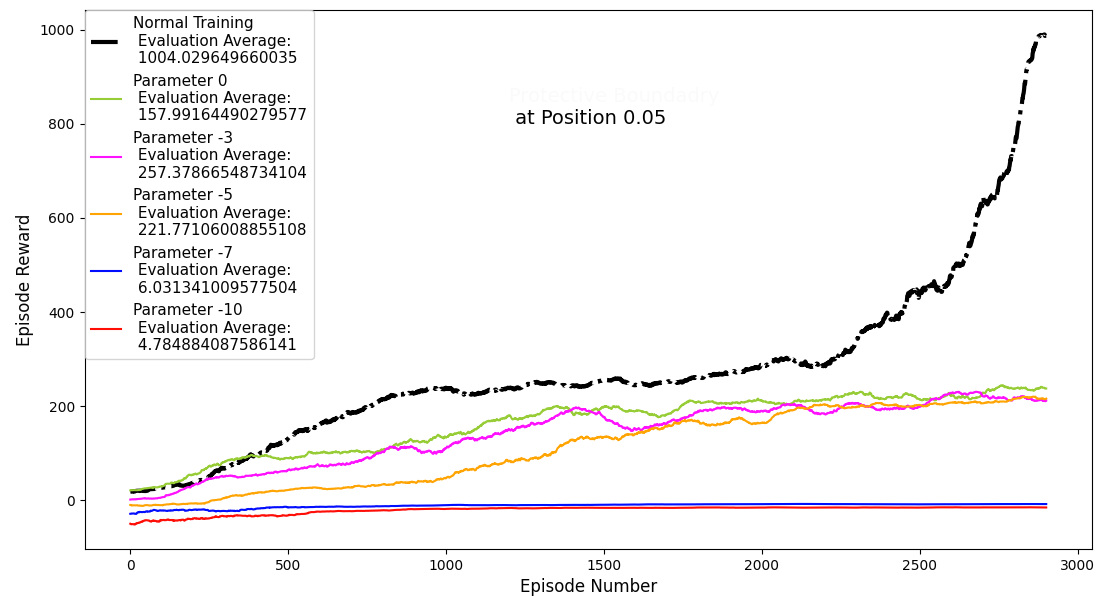
\includegraphics[width=\textwidth]{Hopper_with_Boundary_at_0.05.png}
    \end{subfigure}
    \vspace*{0.0mm}
    \begin{subfigure}[b]{0.5\textwidth}
      \centering
      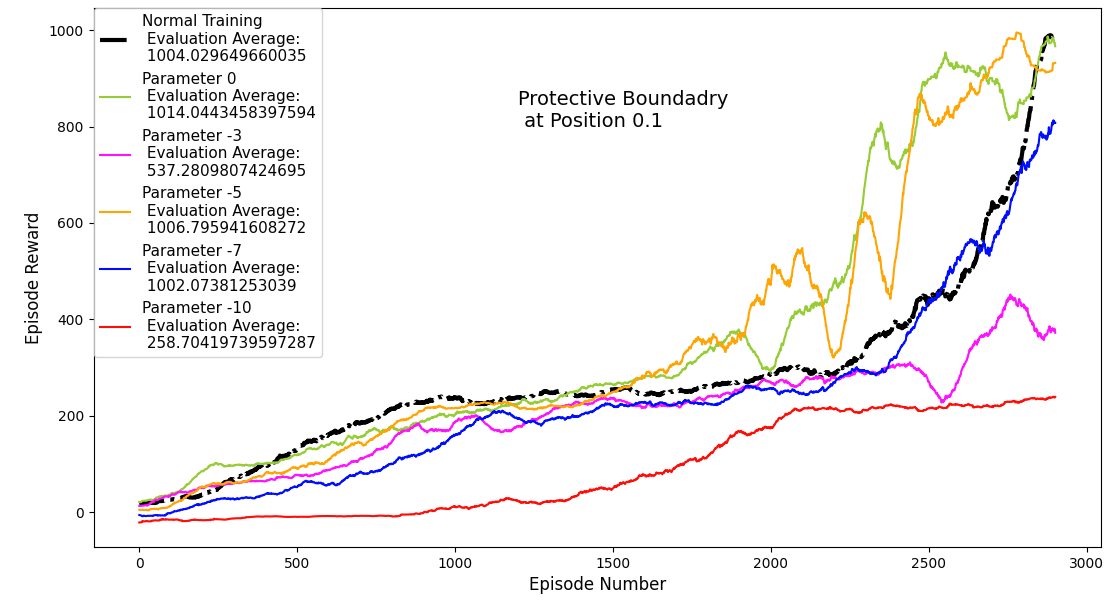
\includegraphics[width=\textwidth]{Hopper_with_Boundary_at_0.1.png}
    \end{subfigure}
    \vspace*{0.0mm}
    \begin{subfigure}[b]{0.5\textwidth}
      \centering
      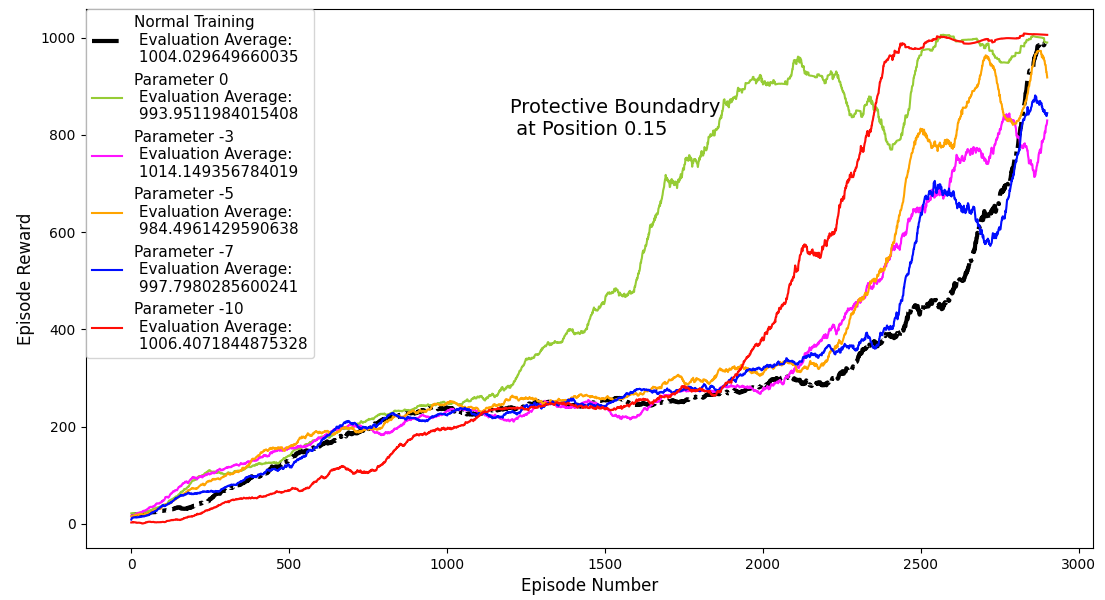
\includegraphics[width=\textwidth]{Hopper_with_Boundary_at_0.15.png}
    \end{subfigure}
    \caption{Hopper}
    \label{fig:Hopper}
\end{figure}


\subsubsection{Walker2d}
fakdflaksdjflakdjflajsdlfjlakdfjlkajdsflkjlasdjf
adfjakjdfhkjahdfkjhasdfkjh
\begin{figure}
    \centering
    \begin{subfigure}[b]{0.5\textwidth}
      \centering
      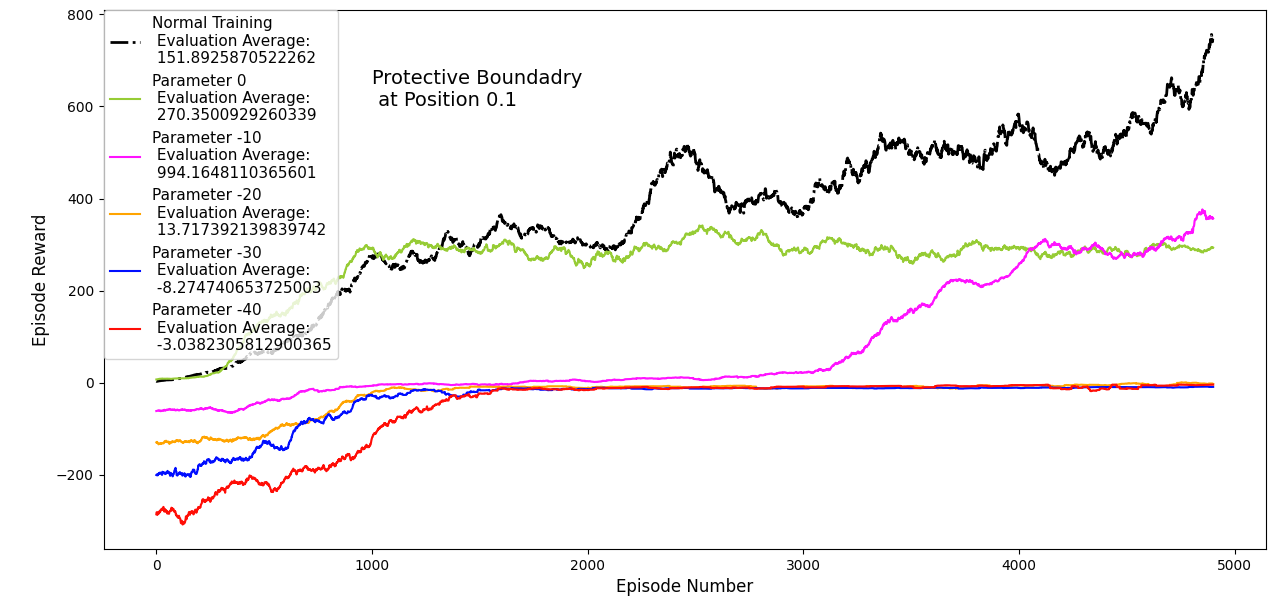
\includegraphics[width=\textwidth]{Walker_with_Boundary_at_0.1.png}
    \end{subfigure}
    \vspace*{0.0mm}
    \begin{subfigure}[b]{0.5\textwidth}
      \centering
      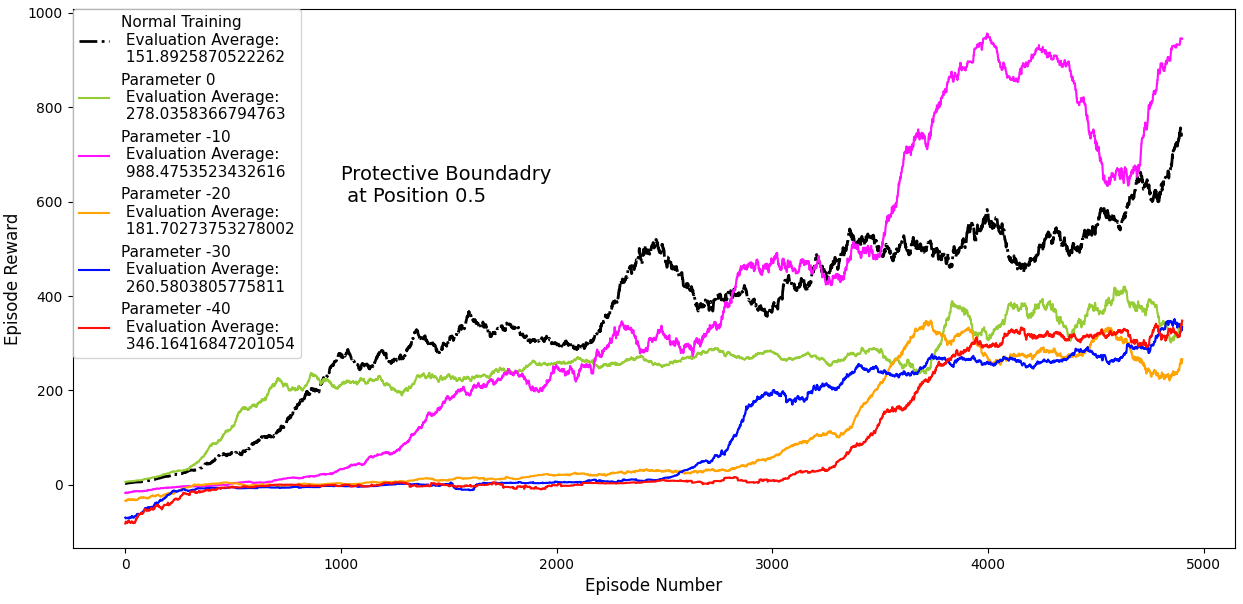
\includegraphics[width=\textwidth]{Walker_with_Boundary_at_0.5.png}
    \end{subfigure}
    \vspace*{0.0mm}
    \begin{subfigure}[b]{0.5\textwidth}
      \centering
      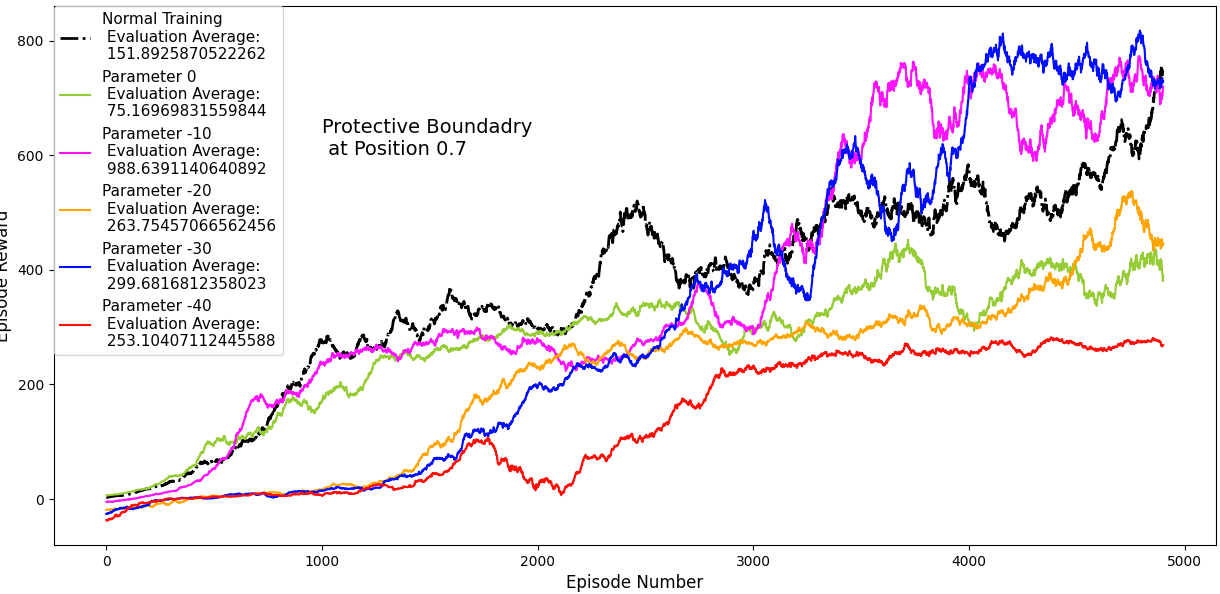
\includegraphics[width=\textwidth]{Walker_with_Boundary_at_0.7.png}
    \end{subfigure}
    \caption{Walker2D}
    \label{fig:Walker}
\end{figure}


\section{Conclution}
As shown by our experiments, when the position and punishing parameter of protective boundary is appropriate, reinforcement learning agent training can be greatly accelerated, much like human atheletes accelerate their acquistion of skills with protective equipments. We have only done experiments on the ones require lower computational power as a proof of concept and we encourage readers of our paper with access to more compute to apply to our idea to enviroments such as humanroid and humanroid standup.

 Our proof of concept data seems to suggeset that when the boundary is set too restrictively, it hinders rather than facilitate learning. Overall, the position of the boundary is more critical compare to penulty parameter, however when the penulty parameter is set too harshly, the learning process can be slowed. The rule of thumb we used during our experiments is that the punishing parameter should be roughly the same as the reward, but with negative sign.

In our experiments, position and penulty parameter of protective boundary is set in a haphazard fashion. Analytical frameworks is required in order to solve this in a systematic manner.

\bibliographystyle{IEEEtran}
\bibliography{Bibliography}
%\printbibliography



\end{document}
